\chapter{Architecture}
    \section{High Level Overview}
        \paragraph{}
        The system is composed of 2 main components
        \begin{itemize}
            \item wslmon - an sdk that contains the detection logic as well as communication logic between kernel-mode and user-mode
            \item wslam - the integrator
        \end{itemize}

        \begin{figure}[H]
            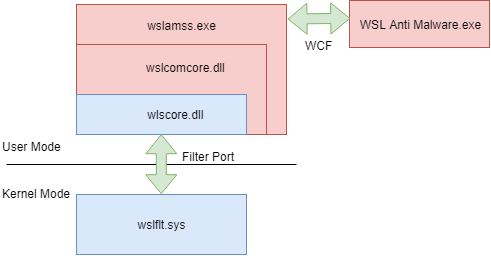
\includegraphics[width=\linewidth]{img/high_level_overview_diagram.png}
            \caption{High Level Overview}
            \label{fig:high_level_overview_diagram}
        \end{figure}

    \subsection{wslmon}
        \paragraph{}
        Wslmon is a software development kit that could be integrated by any OEM to include it in an existing security solution. It consists of:
        \begin{itemize}
            \item wslflt.sys - a minifilter driver that encapsulates the monitoring, analysis and detection logic
            \item wslcore.dll - a shared library that provides an interface to communicate with the minifilter driver
        \end{itemize}
        \paragraph{wslflt.sys}
        is C++ minifilter driver that contains the requirued sensors for monitoring process' activity. It's key components are the
        process filter, file filter, event dispatcher, the communication framework and the detection heuristics.

    \subsection{wslam}
        \paragraph{}
        Integrates the wslmon SDK. It consists of:
        \begin{itemize}
            \item uwpcomm.dll - WinRT
            \item wslamsscomcore.dll - C++/CLI
            \item wslamss.exe - .NET Service
            \item WSL Anti-Malware.exe - UWP Store application
            \item NotificationsListener - Background app service deployed by the WSL Ant-Malware.exe store app
        \end{itemize}
        \paragraph{uwpcomm.dll} uses WinRT in order to send notifications to the background app service via an AppServiceConnection.
        \paragraph{wslammsscore.dll} is built on top of C++/CLI (Common Language Infrastracture) to wrap uwpcomm.dll and wslcore.dll and export managed .NET classes for use
        in the .NET service.
        \paragraph{wslamss.exe} contains the integration logic (ie. exceptions, notifications) and servers as a communication endpoint, built using WCF framework, for
        the store application.
        \paragraph{WSL Anti-Malware.exe}
        is a windows store app that 
        \paragraph{NotificationsListener} is an app service, implemented as a background task, that listens to integrator notifications even if the store application
        is closed, and notifies the user about specific events via toast notifications

    
    %     \subsection{File Filter}
    %     \paragraph{}
    %     The file filter's role is to filter disk I/O.
    % \subsection{Process Filter}
    %     \paragraph{}
    %     The process filter is notified of process and thread creation and termination by the windows kernel.
    % \subsection{Event Dispatcher}
    % \subsection{Communication Framework}
    %     \paragraph{}
    % \subsection{Heurisitcs}
    % \paragraph{}
    % \paragraph{wslcore.dll}
    % is an abstraction of the wslflt.sys driver. It contains the communication logic between kernel-mode and user-mode and exports
    % multiple callbacks to an integrator. It's main purpose is to hide the filtering and detection logic and to provide an easy way to integrate
    % the system in a complete security solution.
